\titre{}
\theme{fonctions}
\auteur{Nathan Scheinmann}
\niveau{1M}
\source{ns}
\type{serie}
\piments{2}
\pts{}
\annee{2425}

\contenu{

\begin{minipage}[t]{0.45\textwidth}{
	\vspace{0pt}
Voici des représentations graphiques de trois fonctions $f,g,h$ de $\mathbb{R}$ dans $\mathbb{R}$.
\begin{enumerate}
\item Détermine à partir de ce graphique:
	\begin{alignat*}{3}
&	f(1)= & \quad \quad \quad \quad&h(1)=&\quad\quad \quad\quad&f(-2)=\\
&g(-2)=&\quad \quad \quad\quad&h(-2)=& \quad \quad \quad\quad &f(0)=\\
&g(0)=&\quad\quad\quad\quad&h(0)=\\
	\end{alignat*}
\item ``Le point $(-49 ;-48)$ appartient au graphe de $h$.'' VRAI ou FAUX ?

\end{enumerate}

	}
	\end{minipage}
	\hfill
	\begin{minipage}[t]{0.53\textwidth}{
	\vspace{0pt}
	\begin{center}
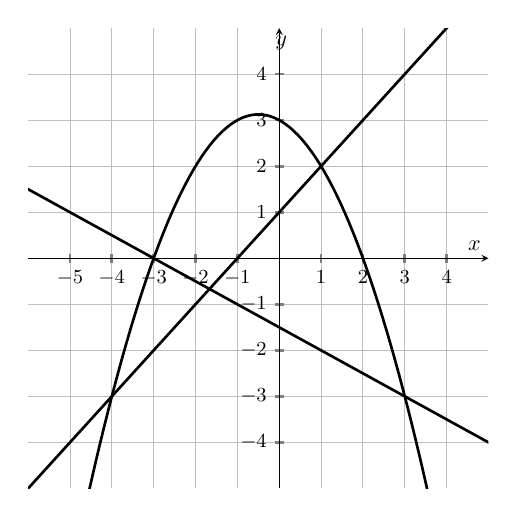
\begin{tikzpicture}[scale=0.8]
\begin{axis}[
  axis lines=center,
  grid=major,
  width=3.5in,
height=3.5in,
  xmin=-5,
  xmax=4,
  ymin=-4,
  ymax=4,
  xlabel=$x$,
  ylabel=$y$,
  enlargelimits={abs=1},
  xtick={-5,-4,...,4},
  ytick={-4,-3,...,4},
  xlabel style={at={(rel axis cs:1,0.5)}},
  ylabel style={at={(rel axis cs:0.52,1)}},
  tick style={very thick},
  ticklabel style={font=\small},
  legend style={
  at={(rel axis cs:1,1)},
  anchor=north west,
  draw=none,
  inner sep=0pt,
  fill=gray!10}
]

\addplot [very thick,domain=-10:10,samples=200] {x+1} node [below right,pos=0.75] {$h$};
%\addlegendentry {$f(x)=...$};
\addplot[black,very thick,domain=-10:10,samples=200]{-1/2*x-1.5}  node[above right,pos=0.1] {$f$};
\addplot[black,very thick,domain=-10:10,samples=200]{-1/2*x*x-x*1/2+3}  node[above left,pos=0.35] {$g$};
%\addlegendentry{$g(x)=...$};
\end{axis}
\end{tikzpicture}
\end{center}	
	}
	\end{minipage}

    \begin{enumerate}
       \item[4)] Complète :
\end{enumerate}
	\begin{multicols}{2}
		\begin{enumerate}[label=\roman*)]
		\item Si $f(x)=-3$, alors $x=$
		\item Si $g(x)=3$, alors $x=$
		\item Si $h(x)=0$, alors $x=$
		\item Si $f(x)=g(2)$, alors $x=$
		\item Si $f(x)=h(-3)$, alors $x=$
		\item Si $g(x)=h(x)$, alors $x=$
\end{enumerate}
\end{multicols}

}
\correction{

}

